\section{Headbanger System Design}
\label{sec:design}

\begin{figure}[t]
\centering
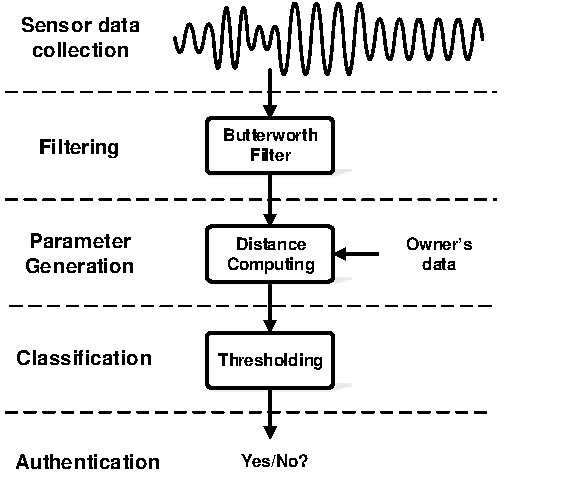
\includegraphics[width=0.75\columnwidth]{figure/system.pdf}
\caption{\systemname~system design flow. The online authentication phase of \systemname~consists of the following steps: (1) sensor data collection in which we collect accelerometer data while users move their head as a response to an audio track played on the glass, (2) filtering in which we apply a Butterworth filtering to smoothen the sensor data for subsequent processing, (3) parameter generation in which we calculate the dynamic time warping (DTW) distances between two accelerometer samples as the parameter, and (4) classification in which we adopt an adaptive thresholding mechanism to classify the user's head movement, whose output will be used as the authentication result.}
\label{fig:sysarch}
\end{figure}

%\begin{figure*}[t]
%\begin{center}
%\begin{tabular}{ccc}
%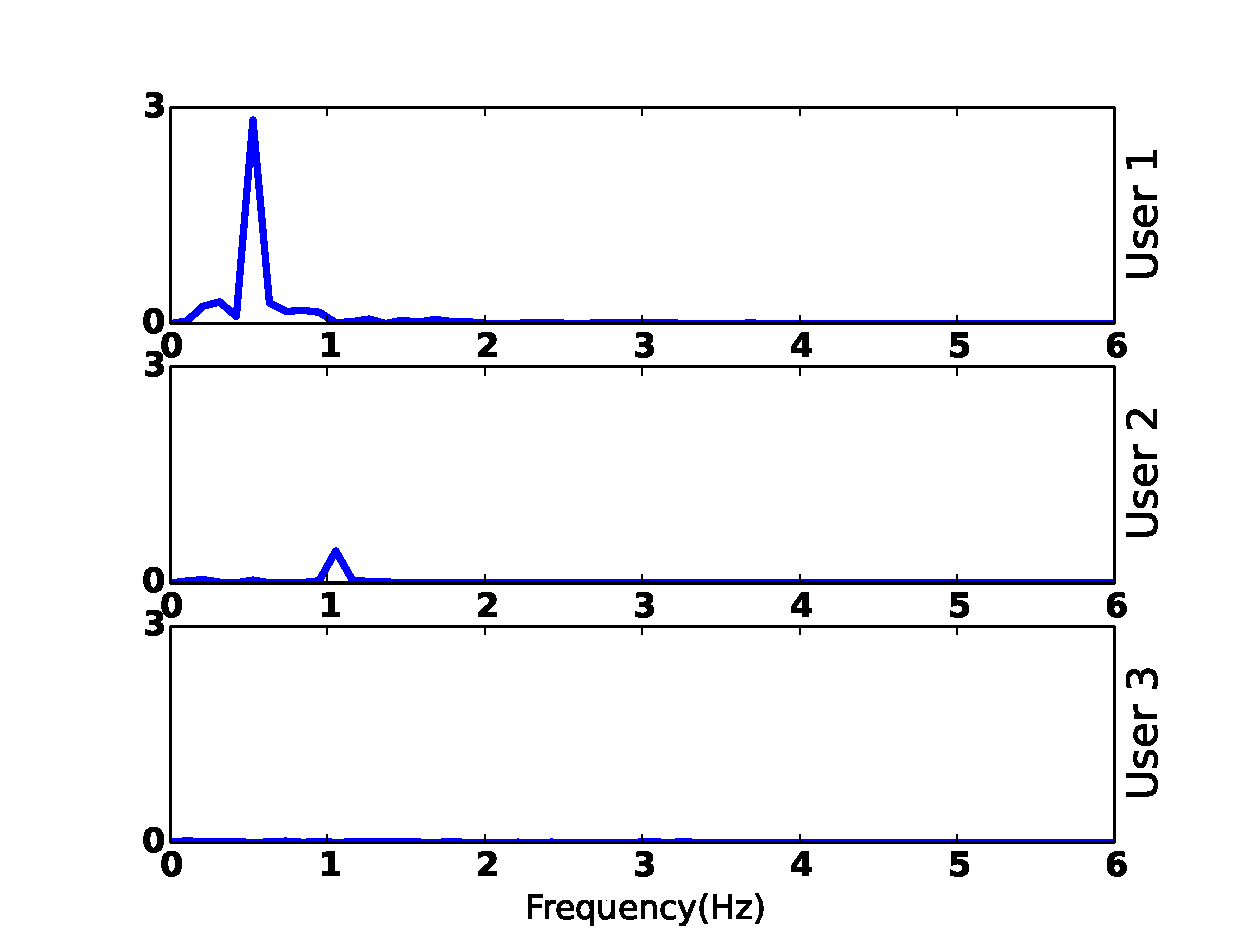
\includegraphics [width=.33\linewidth]{figure/freq_x.eps}&
%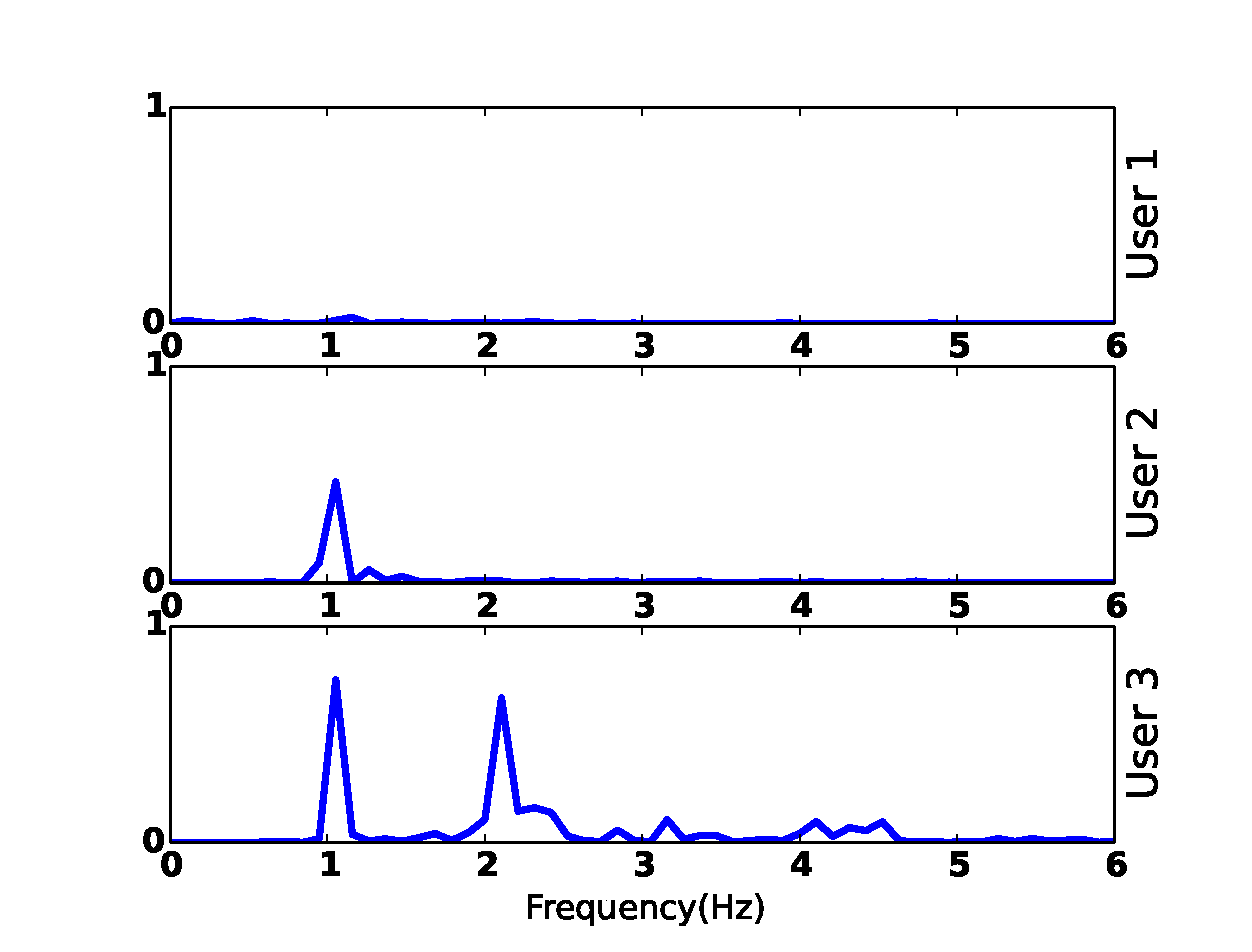
\includegraphics [width=.33\linewidth]{figure/freq_y.eps}&
%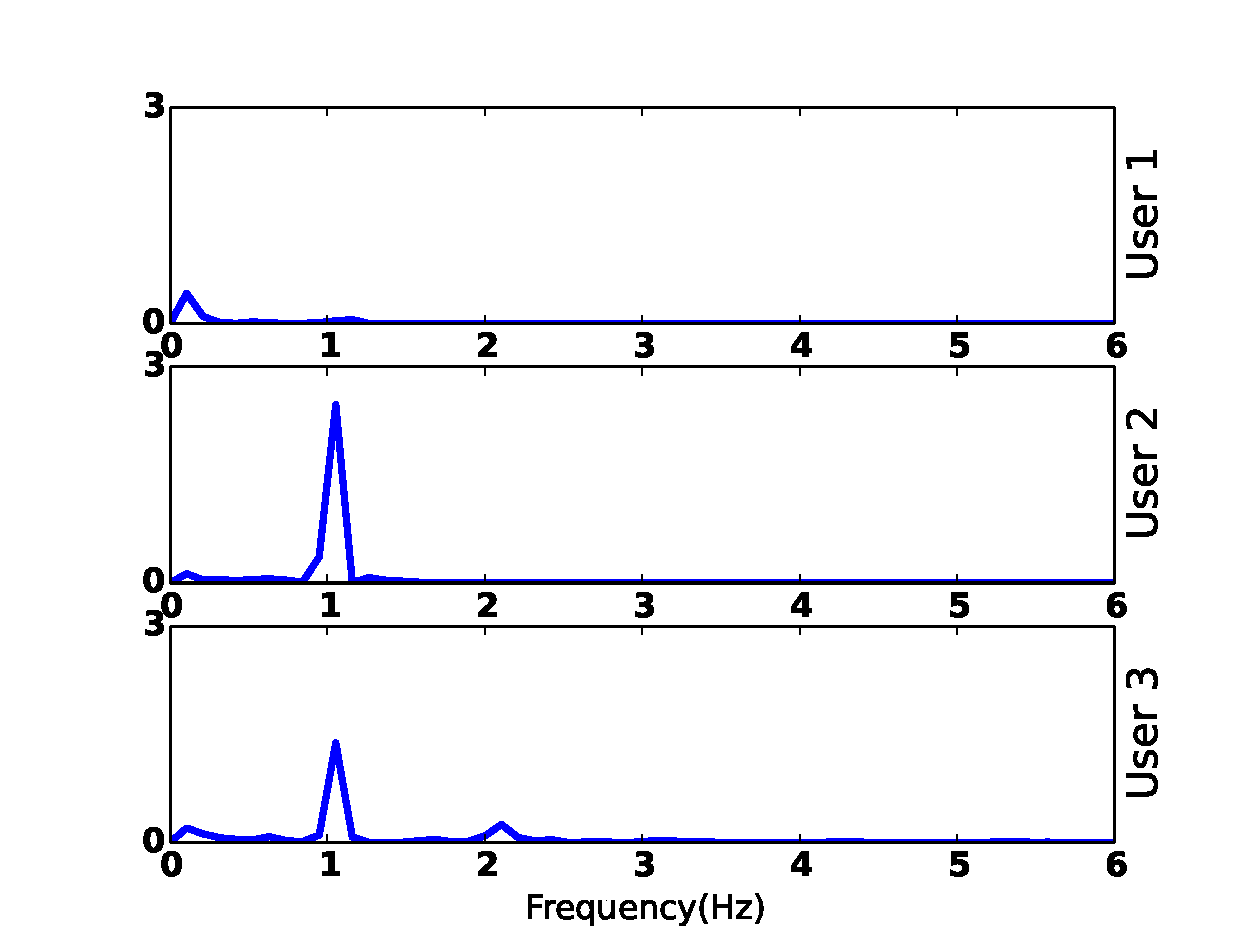
\includegraphics [width=.33\linewidth]{figure/freq_z.eps}\\
%(a) X-Axis & (b) Y-Axis & (c) Z-Axis \\
%\end{tabular}
%\end{center}
%\caption{\label{fig:raw_freq} Accelerometer data from three users, in the frequency
%domain. The data show that the spectrum is significantly
%concentrated within 5Hz for all three users.}
%\end{figure*}

\systemname~enables direct authentication of users to their smart-glass devices or smart-glass apps using
head-movements. We posit that \systemname~will run as a service in the device upon power-up or application start-up,
similar to the screen-lock in smartphones.  %The authentication process is initiated
%by playing a short music cue, to which the user
%responds through head-movements.


 %We envision that our proposed system will be used as an authentication
%interface on the smart-glass wearable device.
The authentication process has two phases: an offline training phase and an
online authentication phase. In the training phase, the system
collects sensor readings when the real user moves her head with a music cue (following her pre-designed movement pattern), and uses the collected data to
build a classifier. In the following discussion, we assume there is only
one real user for the device for the sake of simplicity. An extension to
support multiple users per device can be realized through minor modifications,
namely, by appropriately indexing the users in the trained database.

In the online authentication phase, we collect sensor samples during a user's authentication attempt and label the samples using the \systemname~classifier.
The user is authenticated upon a successful classification.
 %Our design is developed based on the idea that humans respond to music
%naturally through head movements, and that such movements are more
%significant and unique when the track contains fast beats and/or rhythm.
%We will refer to the audio snapshots as {\em music cues} in the rest of the
%paper.
%~\systemname~generates unique features from the head
%movements of a user, and uses them as a unique signature for
%identifying the right user of the device. The system will
%grant access only when the head-movement signature
%generated during the login attempt matches with the
%original user's signature.

As illustrated in Figure~\ref{fig:sysarch}, \systemname~involves the following key modules: sensor data collection and filtering, sample distance computing, and classification.
%\begin{itemize}
%
%\vspace{-2pt}\item {\em Sensor data collection}: ~\systemname~records the head-movements
%in the form of raw accelerometer signals (in 3 dimensions) using the inbuilt
%accelerometer
%sensor on the smart-glass device.
%\vspace{-2pt}\item {\em Filtering}: The accelerometer signals are filtered by applying
%a low-pass filter to remove records of extraneous motion.
%\vspace{-2pt}\item {\em Parameter generation}: The accelerometer signals are
%processed through the dynamic-time warping (DTW) tool~\cite{dtw} to obtain a
%DTW feature that is treated as the unique signature for the user.
%%A user can generate different signatures for different audio tracks. A
%%training phase collects the set of signature for each user-audio pair.
%\vspace{-2pt}\item {\em Classification}: The signatures are classified as
%a match or not a match, based on a thresholding
%scheme and using the trained data set as a reference. The system grants the
%user access to the device if there is a match
%with sufficient confidence.
%%In the former case, the system will grant the user access
%%\item {\em Authentication}: The head-movement signature generated
%%during system operation is compared with the original user-audio pair
%%signature, and the user is authenticated access if there is a plausible match.
%\end{itemize}
%
%The original signature of the glass user is generated through a
%training phase that is executed when the glass is operated
%by the user for the very first time, and the training data gets
%updated upon each use of the device.
%As shown in Figure~\ref{fig:sysarch} shows the block diagram of
%~\systemname system design.
We will now discuss these design aspects in more detail.
\subsection{Sensor Data Collection and Filtering}
%To facilitate natural head movement, we provide several
%short music tracks with easy-to-follow beats.

The data collection step involves collecting motion sensor data (we mainly focus on accelerometer in this study) while the user makes head-movements
in response to the music cue  with a duration of $T$ seconds.
The raw accelerometer
signals are collected at
a sampling rate of $r$ samples/sec. %; the default sampling rate on Google Glass is 50Hz. 
The accelerometer data corresponding to one user,  is a
collection of accelerometer readings on the
3D axis (x, y, and z) collected over $T$-second duration, 
%Figure~\ref{fig:headbanger-illustrate} illustrates the axis
%conventions with respect to the user's head position.
%The data collection unit stores
stored in a matrix with dimensionality $3\times rT$. %where each element corresponds
%to one signal point.
We will refer to this $3\times rT$ matrix as a {\em sample}.
We retain the duration $T$ to be in the order of few seconds, as frequency of
human head movements are, intuitively, typically in the order of few times per
second. %This intuition will be more clear from the filtering stage to be
%discussed next.
%The sensor data is accumulated in a $30r$ matrix, which we refer to as
%one $ACC$ sample.
%We hypothesize that
%head-movement can serve as a reliable behavioral biometric -- that is, $ACC$
%samples from the same user have smaller distances than samples from different
%users.

%\begin{figure*}
%\begin{center}
%\begin{tabular}{ccc}
%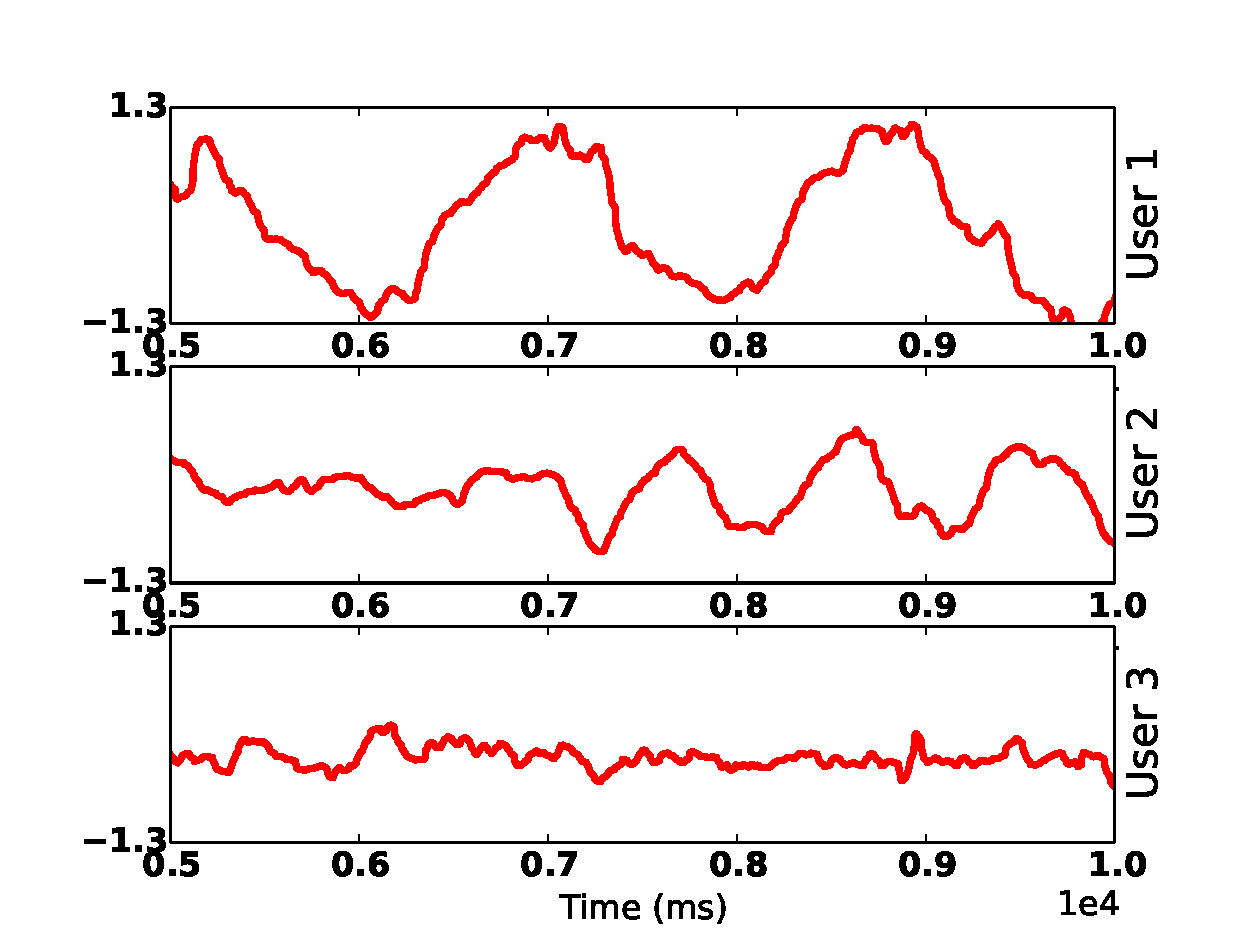
\includegraphics [width=.33\linewidth]{figure/filtered_x.eps}&
%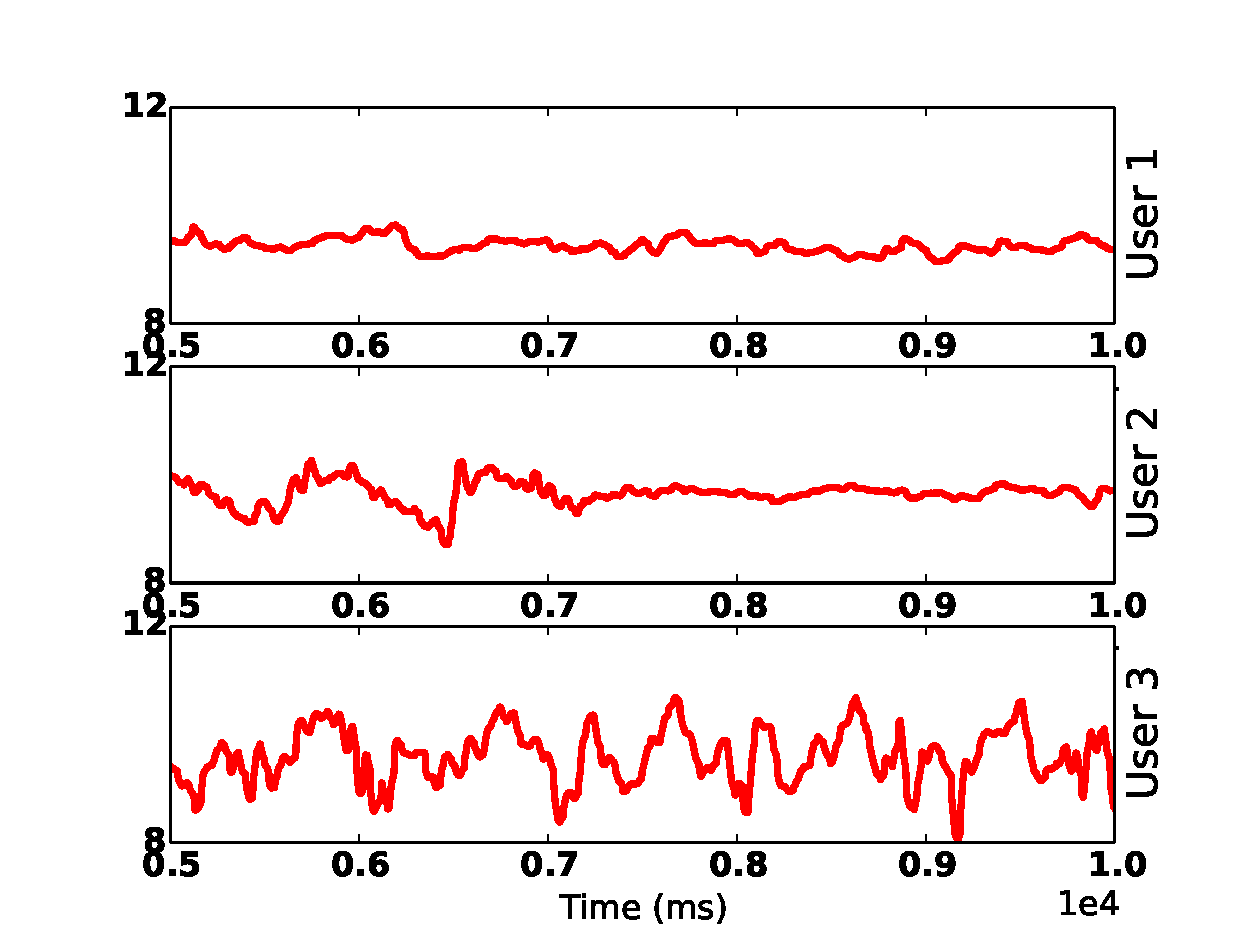
\includegraphics [width=.33\linewidth]{figure/filtered_y.eps}&
%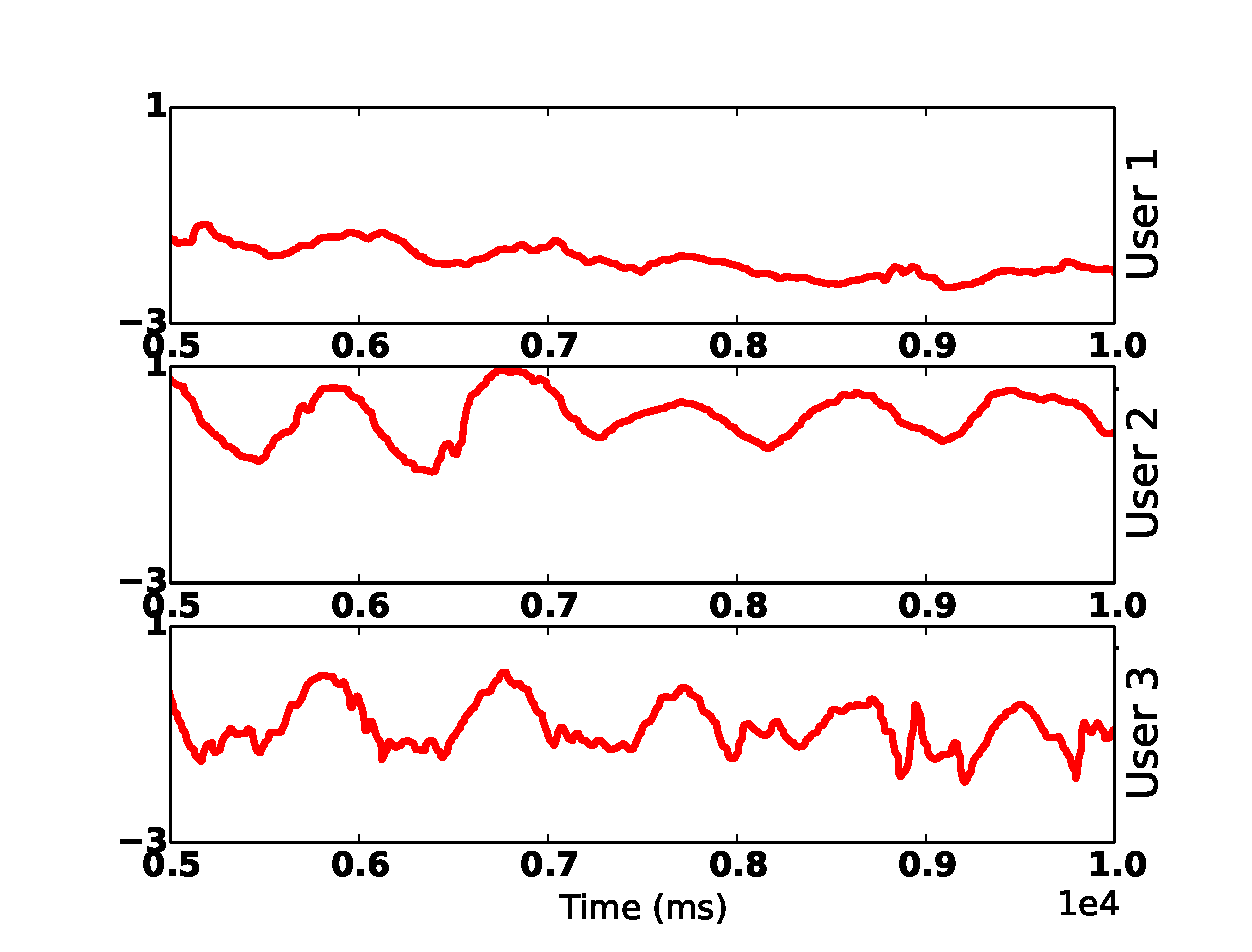
\includegraphics [width=.33\linewidth]{figure/filtered_z.eps}\\
%(a) X-Axis & (b) Y-Axis & (c) Z-Axis \\
%\end{tabular}

%\iffalse
%\begin{tabular}{cc}
%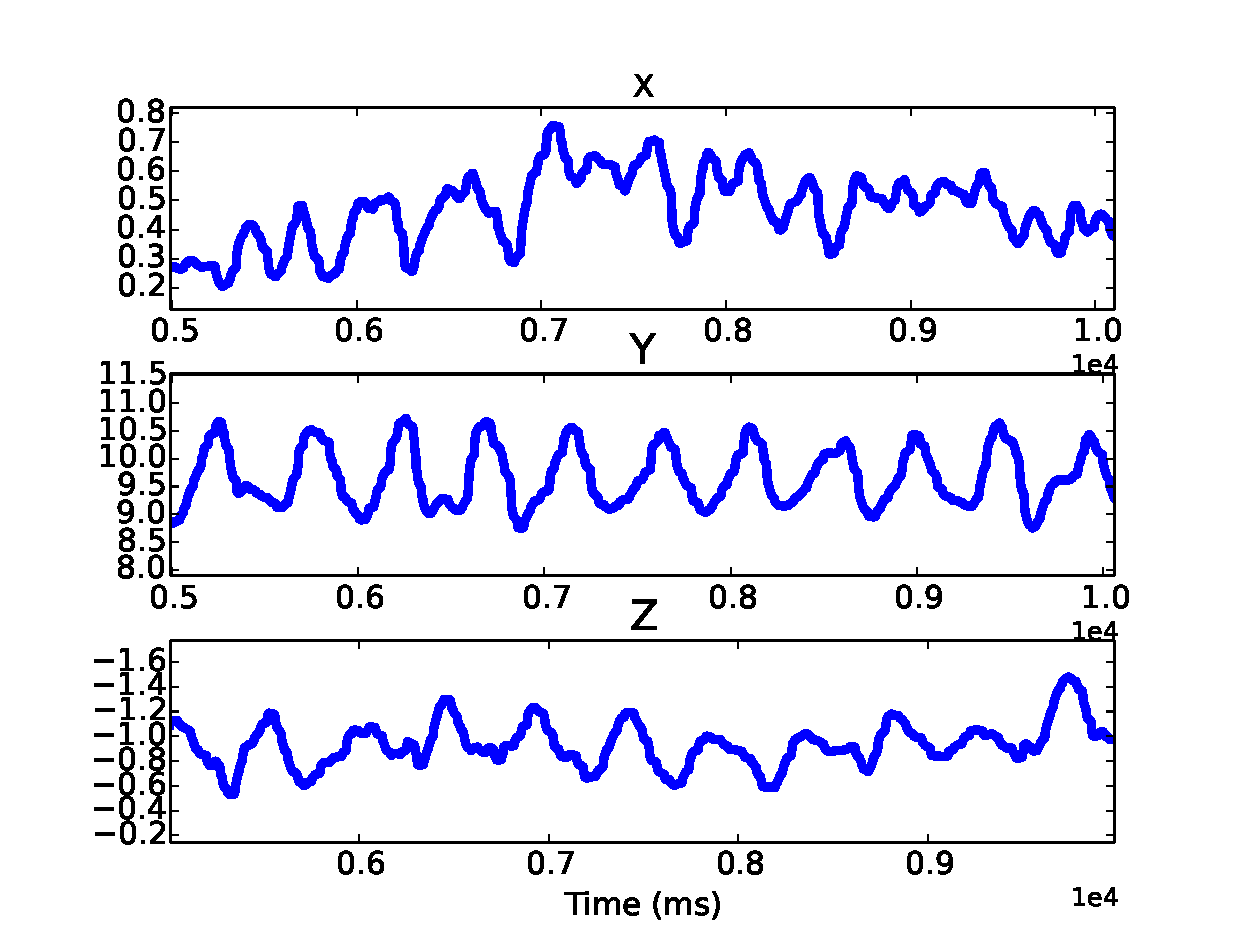
\includegraphics [width=.33\linewidth]{../fig/filer_sub4.eps}&
%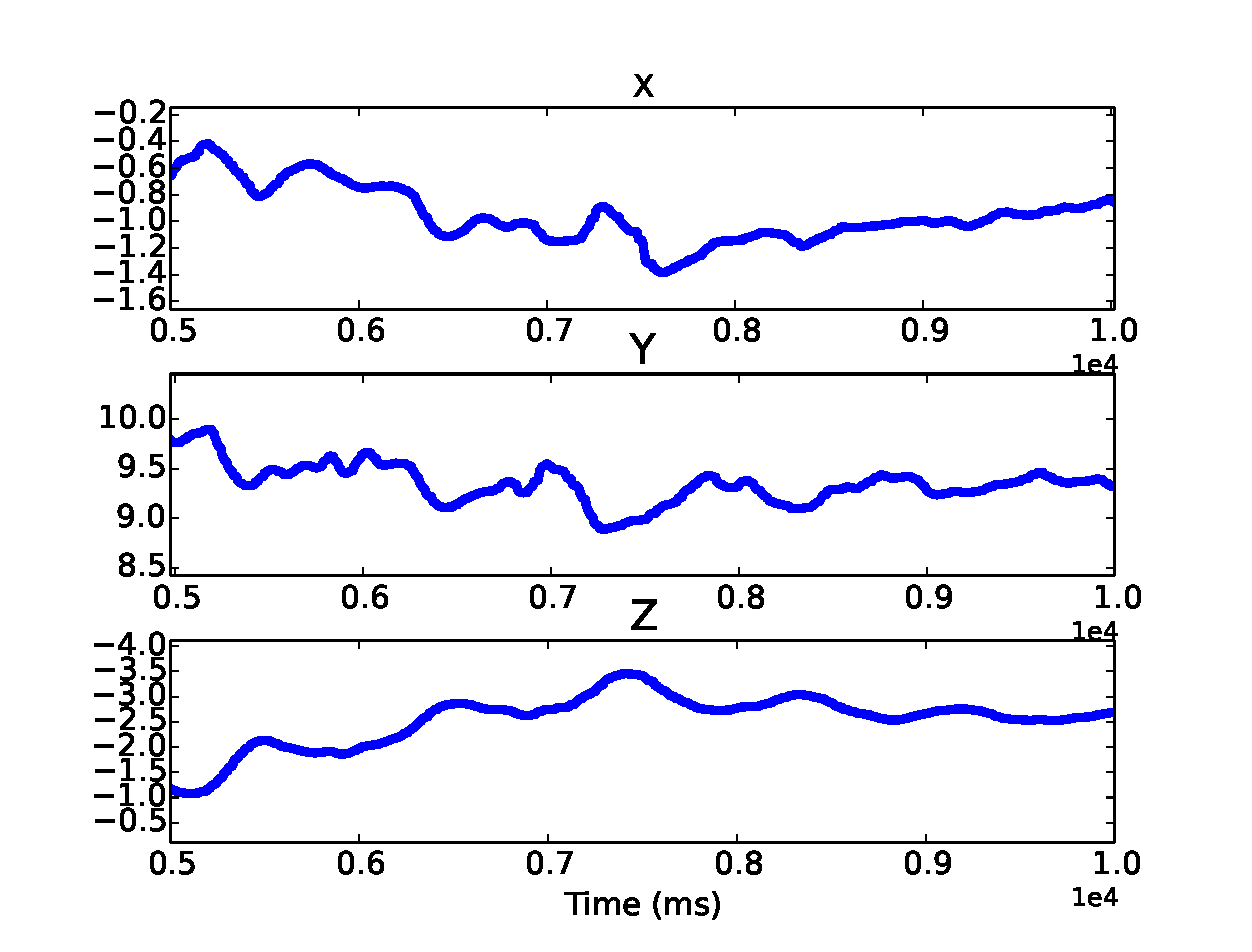
\includegraphics [width=.33\linewidth]{../fig/filer_sub5.eps}\\
%(d) User 4& (e) User 5 \\
%\end{tabular}
%\fi
%\end{center}
%\caption{Filtered accelerometer signals. Applied Butterworth
%filter of order 2 and cut-off frequency 10Hz.
%\label{fig:filteredacc}}
%\end{figure*}


%\subsection{Filtering}

Next, we filter the raw samples to remove noises due to spurious movements such as vibration or shaking.
%The filtering ensures that the head-movement signature
%generated from the accelerometer readings encompasses
%only head movements, and not any spurious signals caused due to
%vibration or shaking.
%From the frequency
%spectrum of each accelerometer sample, as shown in
%Figure~\ref{fig:raw_freq}
%for three users, we can observe that the spectrum is significantly
%concentrated within 5Hz.
%We note that music tracks with high tempo, or fast beats, typically contain
%beats in the order of the order of hundred beats per minute.
%In particular, the high tempo music that we used in our experimentation was
%contained 94 beats per minute~\cite{beats}.
%We infer that the head-movement, in response
%to the beats, will be of the same order. Hence, we hypothesize that
%the signal spectrum in [0,5] Hz range encompass
%human head movements; where 0 Hz can indicate that the head is
%steady still, and 5 Hz can correspond to a vigorous head-shake.
We adopt a low-pass digital Butterworth
filter~\cite{challis1983design} and set a relaxed cut-off frequency of 10Hz.
%Even with the relaxed cut-off, the filtering results in
%clean accelerometer samples with head-movement patterns
%that are prominent and detectable.
%Figures~\ref{fig:filteredacc} (a)-(c) show the filtered results of the raw accelerometer
%samples shown in
%Figure~\ref{fig:raw};
%compared to raw data, the filtered results are much more
%suitable for subsequent processing.

%\begin{figure}[t]
%\centering
%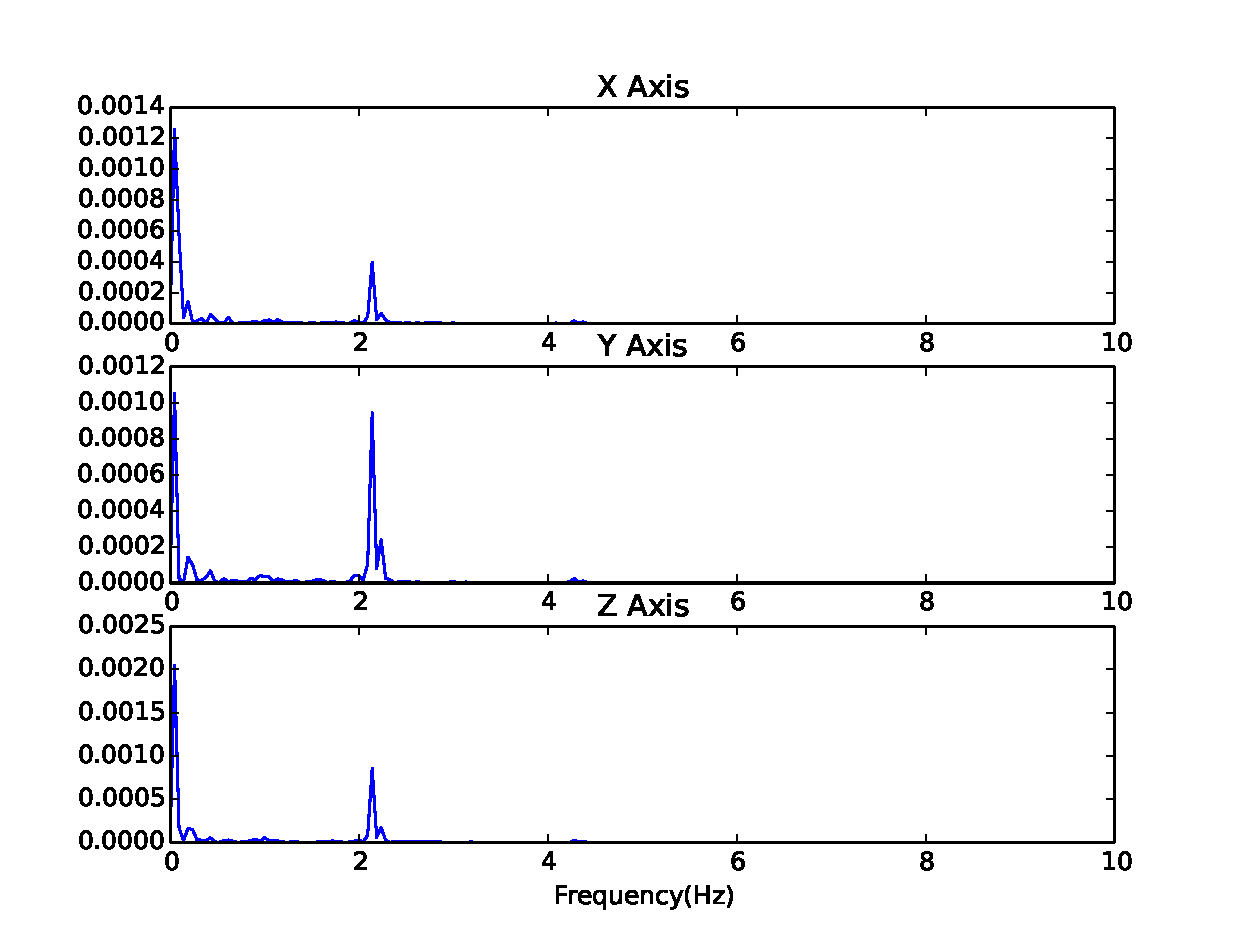
\includegraphics [width=.95\linewidth]{fig/freq_resp.eps}
%\caption{\label{fig:freq_resp}Fiver users' $ACC$ samples in frequency domain.}
%\end{figure}

\subsection{Sample Distance Computing}\label{subsec:distance}
%\subsection{Quantifying Sample Similarity}


In this study, we build a distance-based classifier for its simplicity is well suite for wearable devices. There are various ways of computing distances between two signals; we have considered three popular distance-computing algorithms in this study -- Cosine distance (COS), Correlation distance (COR), and dynamic-time warping distance (DTW).

Suppose we have two time series $S_a = (s_1,s_2, ... ,s_n)$ and $S_b = (s_1, s_2, ..., s_n)$.  Their COS distance is calculated as $\frac{S_{a}\cdot S_{b}}{\left \| S_{a}\right \|\times \left \| S_{b} \right \|}$;   The COR distance is calculated by dividing their distance covariance by the product of their distance standard deviations; The DTW distance is defined as the distance when the optimal alignment between $S_a$ and $S_b$ has been determined by "warping" them non-linearly.   ~\cite{dtw}.
%We generate a signature from the accelerometer signals using the
%dynamic-time warping (DTW) tool~\cite{dtw}. DTW is generally used
%as a similarity matching tool for time-domain analysis of
%temporally varying signals.
%DTW compares a temporal signal with a reference (temporal) signal over a
%certain time-window and yields a distance measure as the score. A low score
%(DTW distance) implies that the test signal is in close match with the
%reference.
%We use the DTW to generate a signature for the head-movements
%from the accelerometer signal.
%We observed from our preliminary tests that, users often
%start head movement at an angle with the vertical which varies among users.
%However, we also observed that the head-movements that follow exhibit a
%consistent, and often periodic, patterns over time.
%We empirically observed that the accelerometer signal patterns
%are consistent after the first 1sec duration of head-movements.
%Treating the accelerometer sample set from the first trial as a reference, we
%apply the DTW algorithm on the successive accelerometer sample set to obtain a
%distance score vector, $\hat{d} = (d_x, d_y, d_z)$; the three elements in
%$\hat{d}$ denote the DTW distance score in the $x, y, z$ axes, respectively.
%By computing the mean of the distance scores obtained for each accelerometer
%pair we generate the mean-value DTW distance, which is treated as the
%head-movement signature or unique {\em feature} for that particular user and
%audio
%combination.

%In the offline training phase, we conduct
%%For evaluation purposes, we conduct an elaborate training phase where
%$M$ trials of head-movement exercises, collect $M$ training samples, and
%obtain $M-1$ reference distance vectors. We observed from our evaluations (to
%be discussed in the next section) that $M = 30$ can yield in high accuracy
%while $M = 10$ can yield reasonable accuracy. The trade off is the computation
%overhead that goes into conducting the training (primarily DTW computations)
%for the $M$ samples.
%In real usage of the application,
%the user would conduct only
%two trials of $T$ duration each where trial 1 is treated as reference.
%In this way, the training can be done in-situ. The training data-set is
%updated upon each usage of the authentication interface.
%%Small distance values DTW is expected to return relatively small distance
%%values for samples from the same user, while returning large distance values
%%for samples from different users (that have different movement patterns).
%%Here, $S1$ is the reference

\iffalse
Next we investigate how we can accurately quantify the similarity level
between two accelerometer samples, whose results will be used to classify the users.
After testing various methods,
We decide to adopt the Dynamic Time Warping (DTW) algorithm that is
often used to measure similarity between two waves based on temporal
stimulation.  Unlike many other algorithms, DTW measures the similarity
between two signals that are similar but with phase difference, which is well
suited for our study. In our study, users often start head movement at a
different angle, but exhibit similar, often periodic, pattern for a similar
amount of time. Applying the DTW algorithm on two accelerometer samples $S1, S2$, we
get a vector $(d_x, d_y, d_z)$ denoting the distance in the $x, y, z$ axes
respectively. DTW is expected to return relatively small distance values for
samples from the same user, while returning large distance values for samples
from different users (that have different movement patterns).

YZ: Sugang, we need some detailed equations or algorithms here.
\fi

\subsection{Classification}
The classification step labels a test sample as ``true'' or ``false'' depending upon whether its distance to the real user's training samples is below a threshold. Again, we choose this method because it strikes a good balance between simplicity and performance. Next, we explain how we build the classifier and how to conduct online classification in detail:
%In this study, we developed a simple yet effective classification scheme based on adaptive thresholds.

\begin{enumerate}

\vspace{3pt}\item \emph{Identifying Top-$K$ Training Samples.} Given $M$ training samples, we first identify the $K$
samples that are closest to all the training samples. For each training sample, we calculate its average distance to the other $M-1$ samples, and then choose those $K$ samples that have the lowest average distance values. These $K$ samples are empirical estimation of the centroid of the sample space, and thus best represent the space among the collection of the training samples. We refer to them as Top-$K$ samples. In our classifier, we focus on the Top-K training samples instead of all the training samples because it does not only incur much less computing overhead, but it also provides much better robustness against noises in training data.

\vspace{3pt}\item \emph{Establishing Distance Threshold.} Suppose a sample, $s$, is one of the Top-K samples. We have its distance scores to the other $M-1$ samples in the training set, from which we can calculate the distance mean $\mu_s$ and distance standard deviation $\sigma_s$. Then sample $s$'s distance threshold is defined as ($\mu_s+n\sigma_s$), where $n$ is referred to as the threshold parameter for our distance-based classifier.

\vspace{3pt}\item \emph{Classifying Test Sample.}   If we use a training sample $s$ to classify the test sample $t$, then $t$ is labeled as a true sample if the distance between $s$ and $t$ is less then $s$'s distance threshold ($\mu_s+n\sigma_s$); otherwise, it is labelled as a false sample. The strictness of this classifier is characterized by
the value of the threshold parameter, $n$; a large $n$ can increase the false
acceptance rate while a small $n$ value can result in a
high rejection rate of true samples. %In our system we aim to reach an optimal
%value of $n$ that can result in acceptable accuracy.
%\item Steps (1) to (3) are repeated when a new sample set is added to the
%training database resulting in an updated threshold. This way, the thresholding
%based classification is adaptive to the user trials. As we will show in our
%evaluations, the thresholding approach is more robust than the SVM approach,
%through both yield reasonable authentication accuracy.

\vspace{3pt}\item \emph{Voting}. We label the test sample according to all $K$ Top-K samples, and the final classification result is the majority decision among all $K$ individual classification results.


%that have
%the lowest $K$ average distance values to the rest of the
%training set. We next calculate their DTW vectors to the rest of the samples in
%the training set to obtain $(M-1)K$ distance vectors. We call this resultant
%vector as Top-$K$ reference distance vector. For example, if $K = 1$, then we
%call the resulting algorithm as Top-1 algorithm; if $K \neq 1$, then we call
%the resulting algorithm as Top-$K$ voting algorithm.
%The voting refers to the procedure that the DTW computation results for each
%sample in the training set is referenced, sorted (in increasing order of DTW
%scores) and the classification (a binary index, match or no-match) is
%performed on the top $K$ entries. The final classification result corresponds
%to the majority vote from the list of $K$ results.
%By using top $K$ samples, instead of all $M$ samples in the training set, we
%significantly reduce the computation overhead in the authentication
%process. In our evaluation, we will study the impact of $K$ value; in
%particular, we evaluate for $K = 1$ and $K = 3$.

\end{enumerate}
Among the four steps outlined above, the first two steps belong to the offline training phase, while the last two steps belong to the online authentication phase.
Finally, if the user's test sample is classified as ``true'' then the user is authenticated to the device; otherwise, the user is rejected.


\iffalse
\subsection{Authentication}

The authentication step results in a binary output that corresponds to
either allowing or disallowing the user to unlock the device.
In this paper, we make two reasonable assumptions pertaining to authentication
on the smart-glass device: (i) homogeneity of
accelerometer sensors for all smart-glasses (from a particular vendor), and (ii)
that the device is registered to the user with an associated PIN or passcode,
and that the head-movement signature is used for secondary verification.
Upon entry of the correct password, the device verifies the identity
of the user based on the head-movement signature.

In the head-movement authentication phase, given a test sample, we classify the sample as true (1) or false
(0) based on one of the two classifiers discussed above. If the result is true, the user is accepted; otherwise
the user is rejected.
\fi

%The authentication mechanism for each of the two classification strategies are
%as follows:

%{\bf SVM.} Given a test sample, classify the sample as true (1) or false
%(0) based on the SVM classifier. %If the result is true, compute the euclidean
%distance between the each of the top $K$ true signatures and the classified
%test signature. If the euclidean distance is below a pre-set threshold
%(obtained empirically from training phase)


%{\bf Adaptive thresholding.} Given a testing sample, calculate the
%DTW distance between the testing sample and the top $K$ representative
%samples. If the resulting distance mean falls within threshold range, then the
%result is ALLOW USER; otherwise, the user is rejected. 